%  ========================================================================
%  Copyright (c) 1985 The University of Washington
%
%  Licensed under the Apache License, Version 2.0 (the "License");
%  you may not use this file except in compliance with the License.
%  You may obtain a copy of the License at
%
%      http://www.apache.org/licenses/LICENSE-2.0
%
%  Unless required by applicable law or agreed to in writing, software
%  distributed under the License is distributed on an "AS IS" BASIS,
%  WITHOUT WARRANTIES OR CONDITIONS OF ANY KIND, either express or implied.
%  See the License for the specific language governing permissions and
%  limitations under the License.
%  ========================================================================
%
\documentclass [11pt, proquest] {uwthesis}[2020/12/20]
\setcounter{tocdepth}{1} 
\usepackage{alltt}  % 
\usepackage[ruled,vlined]{algorithm2e}
\usepackage[table,xcdraw]{xcolor}
\usepackage{adjustbox}
\usepackage{caption} 
\usepackage{rotating}
\usepackage{graphicx}
\graphicspath{ {./images/} }
\newenvironment{demo}
  {\begin{alltt}\leftskip3em
     \def\\{\ttfamily\char`\\}%
     \def\{{\ttfamily\char`\{}%
     \def\}{\ttfamily\char`\}}}
  {\end{alltt}}
\let\mffont=\sf
\begin{document}
\prelimpages
\raggedbottom
\Title{Explorations In Curriculum Learning Methods For Training Contextual Language Representation}
\Author{Daniel Campos}
\Year{2020}
\Program{Department of Linguistics}
\Degree{Master of Science}
\Chair{Shane Steinert-Threlkeld}{Assistant Professor}{Department of Linguistics}
\Signature{Emma Strubell}
\copyrightpage
\titlepage  
\setcounter{page}{-1}
\abstract{Being able to understand language depending on the context of its usage has always been one of the core goals of Natural Language Processing(NLP). Recently, contextual word representations(commonly called language models(LM))like: ELMO, BERT, ELECTRA, and RoBERTA have proven to provide a robust representation of natural language that can be leveraged for a diverse range of downstream tasks. Separately, in many other computer science communities using curriculum learning(CL) methods have proven to be a scalable method of improving model training speed and model performance. While LMs have proven transformational for NLP community the training of these models has proven expensive and difficult. In this thesis we explore the effect of CL in the  training of language models. Using wikitext-2 and wikitext-103 and evaluating word representation transfer learning we find that CL methods produce models can outperform their traditionally trained counterparts  when the training corpus is smaller.}
\tableofcontents
\listoffigures
\listoftables 
\addcontentsline{toc}{chapter}{Glossary}
\thispagestyle{plain}
\begin{glossary}
\item[LM] a language model
\item[Curriculum Learning]
\item[GLUE]
\item[Curricula]
\end{glossary}
 
\acknowledgments{The author wishes to express sincere appreciation to his family, The University of Washington, The City of Seattle, and coffee.}

\dedication{\begin{center}To my wife, Zoe.\end{center}}

\textpages
\chapter {Introduction}
The ability to understand language has long been a fascination for computer scientists worldwide. Early systems like ELIZA \cite{Weizenbaum1966ELIZAA} were designed to interact with humanity through verbal communication. Despite being rudimentary and basic these systems quickly caught the attention of the world and inspired countless researchers to hopefully one day understand and emulate language.  In the decades that have elapsed researchers have grown to understand fundamental concepts about the structure of language and how best to model it. Creating systems that can understand language and preserve its meaning in downstream tasks has long been a focus of the Natural Language Processing(NLP) community. Leveraging deep neural networks researchers have been able to create language representations that represent and understand many of the nuances of human language. These methods have revolutionized nearly every system that works with human language at a pace that seems to be getting faster and faster. These models, despite their impressive performance, are difficult and expensive to create(and recreate) and deploy and it is not clear if there exists a more efficient method to create them \\
In the remainder of this chapter, we first briefly describe the problem we want to tackle and how we will tackle these problems in Section 1.1. Then, we give a brief overview of Curriculum Learning and Language Representations in Section 1.2 and 1.3 respectively. We briefly discuss the goals and challenges of this dissertation in sections 1.4. We then summarize the contributions of this dissertation in section 1.5. We then provide a brief outline of the Dissertation structure in section 1.6 before presenting our statement of originality in section 1.7.
\section{Overview}
This dissertation addresses the topic of the effect of Curriculum Learning methods on Language Models. The term 'Curriculum Learning' refers to a training procedure where the training data for a machine learned method is constructed with a deliberately assembled order with the goal of steering training to a more optimal solution sooner. The term 'Language Modeling' refers to a variety of statistical representations which are used to represent textual language. These methods can be used to understand language and represent language for downstream Natural Language Processing tasks like Question Answering and Information Retrieval. In this dissertation we will explore how curriculum learning methods can be leveraged to improve and create language representations.
\section{Curriculum Learning}
Curriculum's have long been part of the way humans learn. In our schooling instructors assemble information and instruction in a way that allows students to learn foundations and simpler concepts first before they move onto difficult samples. In traditional machine learning for each step of the network learning a portion of the training data is sampled at random. Unlike students in school networks must learn to understand difficult examples at the same time it learns to understand simple examples. There are many formalization's and implementations for curriculum like methodologies in machine learning but for the purpose of this dissertation we will focus on the formalization in frame of neural networks by Bengio et al 2009 \cite{Bengio2009CurriculumL}. In their formalization, curriculum learning is a method for altering the distribution of the training data to allow the network to simpler concepts before difficult concepts.
\section{Representing Language}
In the frame of language understanding researchers have long focused on how to represent all the information which text represents in a way which can be used by other systems. Researchers have explored human curated representations like wordnet \cite{Miller1992WordNetAL}  and explore statistical methods to represent corpuses \cite{Leacock1993TowardsBC}. More recently, statistical methods have tried to produce vector space models where words are represented by a set of vectors in an n-dimensional plane. In the early 2010s, methods like Word2Vec \cite{Mikolov2013EfficientEO} and Glove \cite{Pennington2014GloveGV} were introduced, and the broader NLP community found great leverage in vector based representations of language. Since these word representations mapped each word to a higher dimensional numeric representation systems could now take advantage of the closeness of words via methods like cosine similarity. Moreover, these vector representations of words proved to be a powerful method to represent language for many downstream tasks like: Information Retrieval, Question Answering, Sentiment Analysis, Machine Translation, etc. \\ 
These fixed word vectors drove incredible improvement and research across many fields but since representations focused on word level vector values, systems were unable to represent word as it different in context. For example: the word fly was represented by the same vector independent if the context was dealing with an insect (There is a fly in my soup!), an action (I want to fly away.), or a description of personal style(You sure look fly!). To expand word representation out of discrete words researchers explore methods like having multiple word vectors for each meaning of a word \cite{Hu2016DifferentCL}, sentence vectors \cite{Kiros2015SkipThoughtV}, paragraph vectors \cite{Le2014DistributedRO}, Gaussian mixtures \cite{Athiwaratkun2017MultimodalWD}  and sub word vectors \cite{Bojanowski2017EnrichingWV} all with the goal of improving models ability to capture expressive semantic information and performs better in situations with polysemy. Many of these techniques were very similar to word vectors but tried to represent all sentences in a corpus using a fixed size vector. While these techniques also drove vast improvement in NLP tasks they struggled to represent sentences outside of the original training corpus and minor changes in sentence structure could have a large effect on the vector representation. \\
As part of these explorations, researchers used Language Models(LM) to learn word representations. Language modeling is a well defined NLP problem that aims to model a statistical distribution of words in a sentence so we can for some type of prediction about next word. Using LM systems with sesame street inspired names like: ELMO \cite{Peters2019KnowledgeEC}, BERT \cite{Devlin2019BERTPO}, ERNIE \cite{Sun2019ERNIEER} were able to produce what could seem like a never ending stream of new State-of-the-art(SOTA) models that excelled at most NLP problems. The success of these models spun a seemingly continuous wave of new techniques building of BERT like KnowBERT \cite{Peters2019KnowledgeEC}, RoBERTa \cite{Liu2019RoBERTaAR}, AlBERT \cite{Lan2019ALBERTAL}, ELECTRA \cite{Clark2020ELECTRAPT}, and BART \cite{Lewis2019BARTDS}.  \\
While these deep learning based LMs have shown to be great methods to enable language understanding in many tasks, the ability to train these models is becoming increasingly computationally expensive. 
\section {Goals and Challenges}
The goal of this dissertation is to explore how curriculum learning effects Language representations. First we explore methods for evaluating the difficulty of a sentence. Using difficulty scores we then explore how to use this difficult to develop and train models with a curriculum. The final of this dissertation is to evaluate the wide spread of curriculum methods in a way that we can draw conclusions which are representative for usage on all language models.
The main challenge in this dissertation is to scope the work to allow us to gain maximum feedback cycles. Since training large language models requires a lot of computation doing an exhaustive exploration of both curriculum methods and tuning doing an intensive hyperparameter sweep for each model would be too time intensive. Ensuring our work is representative to variations in model size and dataset size will also be challenging. Finally, ensuring our work is reproducible and expandable will also be a challenge.ks. 
\section{Contribution}
Our contributions are threefold: we find that LM performance as measured by perplexity on the training corpus is not a predictive measure of transfer learning performance, CL method can produce better contextual word representations on smaller corpuses but as corpus size scales CL methods produce worse models, and we find that random curricula can prove to be as good curricula as linguistically motivated curricula.
\section{Structure of This Dissertation}
In Chapter 2 we present the background material in system architecture Curriculum learning, Language Modeling, and methods for evaluating Language Models. For Curriculum learning, we give a detailed and technical introduction to Curriculum Learning and discuss some recent applications in the NLP domain. With regard to Language modeling, we introduce the concept of language modeling, describe various methodological advances and improvements discovered over time, and contrast various implementations. We will also provide a brief introduction to the effects of large language models and why focusing on model training efficiency is important. Finally, we introduce some of the most popular methods for evaluating language modeling along with the datasets and frameworks we will use for our experiment. \\
In Chapter 3, we provide a detailed explanation of our experimental setup. We propose two curriculum learning strategies building on prior work and explain how we implemented these strategies and how we evaluate the effectiveness. 
In Chapter 4, we discuss the results of our experiments along with a broad analysis of the impact our various methodologies had on model performance.
In Chapter 5, we conclude this thesis.
In Chapter 6, we discuss future work we would like to research.
\section{Statement of Originality}
I declare that this thesis was composed by myself and that the work it presents is my own, except where otherwise stated.
\chapter{Prior Work}
In the previous chapter, we briefly introduced the basic ideas of Curriculum Learning and Language Modeling(LM). In this chapter, we provide a fuller treatment of these areas. In particular, in section 2.1, we describe the building blocks many language models use. Then, in section 2.2 we give a technical overview on Curriculum learning methodology focused on its implementations in Machine Translation. In section 2.3 we provide a technical overview on Language modeling focusing on how many recent systems have structured the problem and the effect various implementations have on downstream performance.  Finally, in section 2.4 we introduce a suite of evaluation frameworks which have become the de facto. quality of language model standard.
\section{Architecture}
\label{chap:prior:sec:arch}
In this section, we first briefly review of neural networks in NLP in \fullref{chap:prior:sec:arch:nn} so as to obtain insight into how system architecture can effect downstream tasks. Then, in section \fullref{chap:prior:sec:arch:lstm} we introduce Long Short Term Memory(LSTM) \cite{Hochreiter1997LongSM} and describe how it works. In section \fullref{chap:prior:sec:arch:transformer} we introduce the Transformer \cite{Vaswani2017AttentionIA} and briefly discuss how it differs from LSTM.
\subsection{Neural Network in NLP}
\label{chap:prior:sec:arch:nn}
In the last few decades, neural networks have provided language researchers with an effective method of building models that represent the complex phenomena associated with language. In NLP, Recurrent Neural Networks (RNN) are popular building blocks because they can retrain contextual information from previous states. While useful, RNNs are limited in their ability to understand a full sequence by their short-term memory. When presented with long sequences of input, the amount of information needed to understand the total input and how individual components relate grows. Since this state is limited in size as sequences get more prolonged, less context about particular parts of the sequence is kept in the hidden state. The slow loss of prior input's information can be incredibly impactful for textual representations where coreference can be many sentences apart. Besides issues in representing inputs with large context windows, RNNs suffer from what is known as the vanishing gradient problem \cite{Hochreiter1998TheVG}. The vanishing gradient problem focuses on how, when training RNNs, we must update the weights of previous hidden states, but as we do so, their gradients get smaller and smaller. Eventually, the gradient on earlier weights is so small that it practically vanishes, and older weights are not updated. To address this shortcoming and improve modeling long term dependencies architectures like LSTM and the Transformer were introduced. 
\subsection{LSTM}
\label{chap:prior:sec:arch:lstm}
The LSTM was proposed by Hochreiter et al.,  1997 \cite{Hochreiter1997LongSM} as a neural method that did was able to avoid vanishing gradients. LSTMs have a gating mechanism that regulates the flow of information from previous states into the current state. What makes the LSTM unique is that it has forget gates that are trainable parameters which choose what information from earlier parts of the input is forgotten. Using these gates, LSTMs can retain relevant information even with large input sizes. Since LSTMs excel at data where their long term dependencies, they have revolutionized the world of time-series prediction \cite{Sagheer2019TimeSF}, speech recognition \cite{Han2017ESEES}, and neural machine translation (NMT) \cite{Jean2015OnUV} to name a few. 
\subsection{Transformer}
\label{chap:prior:sec:arch:transformer}
The Transformer is a neural system first proposed by Vaswani et al., 2017  \cite{Vaswani2017AttentionIA} as a system for NMT. The transformer block introduced a way to move from RNNs to an architecture that focuses on the interaction between units in the input data. Attention is a method that selects what portions of the input are related to each other. Instead of keeping a global state like an RNN, Transformers focus on distilling what input items are attended to by other parts of the data. Attention is a learned weight mechanism that represents how much one item in a list is related to others. In NLP, this method has been extremely successful as it allows a model to learn the interdependence of terms without any pre-processing. In its initial formulation, the implementation had an encoder and a decoder, consisting of 6 stacked transformer layers. All encoders are identical (but do not share weights) and have two sub-layers: self-attention and a feed-forward network. All decoders are identical(and do not share weights) and consist of 3 sub-layers: self-attention, encoder-decoder attention, and a feed-forward layer. \\ 
Vaswani et al., 2017 use multi-head attention to produce a linear projection used to attend to different parts of the input. Since this method does not rely on recurrence or convolution, a positional encoding is introduced to understand where in a sentence a word is. For more details about the mechanics of the Transformer, we recommend reading The Illustrated Transformer\footnote{https://jalammar.github.io/illustrated-transformer/}. In the original implementation,  stacked layers of transformers train translation systems for English to French and English to German translation, which results in new SOTA models with $\frac{1}{4}$ the training time. \\
The Transformer's ability to model long-term dependencies well and efficiently has made it a natural fit for most NLP tasks. As we will cover in succeeding sections, researchers have used this method to produce robust and usable language representations.
\section{Learning Methods}
\label{chap:prior:sec:cl}
In this section, we first briefly review some learning methodologies for neural networks in Section \ref{chap:prior:sec:cl:overview} to formalize what learning methods seek to achieve. Then, in Section \ref{chap:prior:sec:cl} we provide a more in-depth description of curriculum learning and cover some ways it has been using in NLP. 
\subsection{Brief Overview of learning methodologies}
\label{chap:prior:sec:cl:overview}
Neural Networks are usually trained by randomly selecting batches of data in a training corpus. This method has proven to be incredibly robust as it allows the model to learn the data distribution gradually. While useful in eventually learning data distribution, random sampling is unable to build any natural hierarchy or structure quickly. Methods like Curriculum Learning \cite{Bengio2009CurriculumL}, reinforcement learning \cite{Sutton1998ReinforcementLA}, and active learning \cite{Cohn1994ActiveLW} are alternative methods which try to improve model training and accuracy by sampling training examples in a non-random way. Most methods at their core seek to optimize what kind of information a model has access to at each step in training to find better gradients than a random sample. In domains like Generative Adversarial Networks (GAN) \cite{Goodfellow2014GenerativeAN}, training models that generate large images has proven difficult. GAN is a machine learning framework where two NNs, a generator and a discriminator, compete in a zero-sum game. The discriminator, seeks to classify samples as real or synthetic (created by the generator) while the generator, seeks to creates artificial samples which are close to sample from the training dataset. What is unique about GANs is the generator's goal is not to produce an sample that is similar to some real sample but produce a sample which fools the discriminator. This methodology has proven incredibly effective in producing realistic photos and other complex synthetic data in an unsupervised way. Finding structure in the size of images, researchers have found tremendous improvements by slowly increasing the target output size as training progresses \cite{Karras2017ProgressiveGO}. Initially, the Generator produces 2x2 pixel images. Once it and the Discriminator converge, the target output size is increased to 4x4. This method of scaling continues until 4096x4096 pixel images are synthesized. By training in an increasingly entropic way, the final model can learn a better representation with a higher sample efficiency. This work on progressive learning in GANS inspired this dissertation as LMs, much like GANs, are conceptually simple but can prove difficult to train at scale. 
\subsection{Curriculum Learning}
\label{chap:prior:sec:cl:cl}
While the common usage of CL in computer science begins in 2009 \cite{Bengio2009CurriculumL}, the concept of CL is much older. At its core, CL's vision is the idea of choosing examples to be presented in a specific order to guide the agent to learn quicker than if they had seen samples in random order. Early experiments with RNNs \cite{Elman1993LearningAD} focused on learning grammar suggested that learning of complex grammatical structure improves when the initial examples the models learn with are more straightforward. CL guides the optimization process to converge faster and guide the learner to better local minima and can be thought of as a method of re-weighting the data distribution over model training. Unlike CL, regular random batch sampling emphasizes an equal contribution of each data point without any notion of how common the data point is and if the data point can be used to build a foundational understanding.\\
In their 2009 paper \cite{Bengio2009CurriculumL}, Bengio et al., 2009 suggest that CL approaches training may act similarly to unsupervised pretraining. The authors explore the effect of CL in three experiments: using a perceptron to learn an equation, shape recognition, and language modeling. In their language modeling task, they modify the training corpus to make it increasingly difficult. This language model is trained using samples with a windows size of 5 tokens sampled from the 631m token Wikipedia corpus. Initially, they remove samples which contain any word that is not in the N most common words (starts with 5,000). After each pass on the corpus, N is increased by 5,000 which means the training corpus gradually gets larger, more difficult, and more representative of the full corpus distribution. After 1 billion updates, the CL method has a loss of 2.78 vs. the non-CL loss of 2.83. The two main issues in CL are: the computational cost to assemble the batch and the significant amount of data the model can learn from in early epochs is low. \\
Since this original paper, CL methods have proven effective for many NLP domains, especially in NMT. Wang et al., 2019 \cite{Wang2019LearningAM} expand on the idea of CL as a method of data selection and data augmentation. Their implementation focuses on selecting data relevant to all tasks and disregarding data that may be only applicable to a specific domain and can bring a 2.5 BLEU point improvement vs. non-curricula implementation. Platanios et al., 2019 \cite{Platanios2019CompetencebasedCL} introduce the notion of competence-based CL, which is the basis for much of our experimentation. The author's main contribution is building a CL method called competence curricula, which only controls how long the curriculum lasts before regular training occurs. The authors' approach is 2-stepped: assign a difficulty value to each sample in the training data, and train the model with increasingly more data as its competence improves. In the first stage, a heuristic is applied to rank the training data from easiest to hardest. Using a cumulative density function (CDF), each sample is then given a value from 0 to 1, which equates to how difficult the example is. Then, starting with some initial competence $\lambda_0$, the model will train by sampling a training batch from the training data where the sample difficulty is lower than the model's current competence. After each batch is sampled, the model's competence is increased by some step $\epsilon$ until it is training on the full dataset. A more detailed description as it applies to this dissertation can be found in Chapter \ref{chap:method}. In their experiments on NMT, the authors explore the effect of competence-based CL using Transformers and BiLSTMs using two difficulty methods (sentence length and word rarity) and two competence step functions (root and linear) and find that all of their CL implementations outperform their non-CL counterparts. Using the competence curricula method, the Platanios et al., 2019 can reduce training time by up to 70\% and improve BLEU performance by 2.2 points on the WMT dataset compared to non curriculum methods. 
\section{Language Modeling}
In this section, in section 2.2.1 we briefly review of what language modeling is, various methodologies, and why language modeling is so useful for NLP. and then explore why its relevant for NLP.  Then, in section 2.2.2 introduce ELMO followed by BERT in 2.2.3. Then, in 2.2.4 we discuss some other major LMs and how the broader NLP community is using them. Finally in 2.2.5 we discuss some of the effects of large LMs to ground the motivation of our research.
\subsection{What is Language Modeling}
Language modeling is a way to assign a probability distribution over some textual representation. In other words language modeling is an application of conditional probably, E.G. $P(w_{1},\ldots ,w_{m})P(w_{1},\ldots ,w_{m}) $ where $w_i$ is a word in a sentence. Language models can be useful methods to represent natural language because they allow models to differentiate meanings of sentences based on context. In other words a model is able to understand that the word 'fly' can mean different things in the sentences: "You look fly", "Lets fly away!", "That is a fly". \\
While language modeling is by no means a new concept it was not until the introduction of Neural Network based LM that these representations were able to serve as general understanding frameworks. Prior to these Neural Network Language Models(NNLM) language modeling usually focused on modeling some some form of an n-gram where the probability of a word only depends on the previous n words. Large Neural Network based LMs are usually used as the first step in a NLP application as a way of turning some form of textual input into a representation in a vector space.
Language models can be created using many training objectives but in general models tend to be either auto encoding or auto regressive. Auto Encoding models seek to learn an efficient representation for language through training the signal to ignore data. Auto regressive models learn language by building language into conditional probability with the logic that if a model learns to predict previous or next words it must be able to predict language given context.
\subsection{ELMO}
ELMO was introduced by Peters et' al 18 \cite{Peters2018DeepCW} and in many ways became the first contextual word representation that saw widespread usage. The name ELMO represents Embeddings from Language MOdels and is a reference to how language modeling can be used to train contextual word embeddings. ELMO is an auto-regressive model built off the success of GloVe \cite{Pennington2014GloveGV} and Word2Vec \cite{Mikolov2013EfficientEO} by seeking to be the first stage of textual processing for a variety of NLP tasks. ELMO consists of a character-level convolutional neural network(CNN) followed by two layers of bidirectional LSTMs. The CNN is used to convert words from a text string into raw word vectors which are then passed to the BiLSTMs to model the whole input. By using a character level CNN ELMO is able to capture the inner morphological structure of words, e.g. words like beauty and beautiful are similar when character level convolutions are used.\\
Each layer receives a forward pass and backward pass over the textual input which allows the model to read the sentence left to right and right to left and form representation that understand the whole context of a sentence. The forward pass of the text(reading left to right) allows the model to build context for a word given previous words while the backward pass(reading right to left) allows the model to build context from the end of the input to the word being modeled. The backward and forward pass are concatenated together. The output of the first biLSTM is passed into the second layer and then the final ELMO representation is the weighted sum of the raw word vectors and the 2 intermediate word vectors(outputs of each biLSTM).\\ 
The ELMO model was trained by using the Billion Word Corpus \cite{Chelba2014OneBW} and using the unprocessed input as the target for ELMO's language modeling task. The model is trained for 10 epochs(complete passes on the corpus) which takes approximately 3 weeks using 3 1080ti GPUs. On average the authors find that adding ELMO as a text representation layer provides 20\% improvement across a diverse set of NLP tasks.
\subsection{BERT}
Building on the success of ELMO, leveraging the transformer architecture \cite{Vaswani2017AttentionIA}, and taking the leanings from other contextual word embeddings \cite{Howard2018UniversalLM} \cite{Radford2018ImprovingLU} Devlin et. al 18' introduced BERT which stands for Bidirectional Encoder Representations from Transformers. BERT seeks to model language by being an auto encoder that uses modified stacked transformer encoders (12 layers for small model and 24 for large) to build a contextual language representation. Instead of using character level convolutions or fixed word vectors as a starting point BERT leverages a piecewise tokenization \cite{Wu2016GooglesNM} which sets a vocabulary size of  30,000 which allows BERT to exploit the natural morphology in language.  \\
Just like other language models before it, BERT uses unsupervised pre training on a large text corpora to train the model. Unlike previous models BERT introduces two new training objectives as a way to steer the model: Masked Language Modeling(MLM) and next sentence prediction(NSP). 
MLM reformulates the language understanding as a cloze task \cite{Taylor1953ClozePA} where the models goal is to predict what a hidden word in a sentence may be. To train using MLM BERT introduces a new token '<MASK>' to represent the hidden word. 15\% of each the corpus tokens are selected to be replaced of which 80\%(12\% of the corpus) are replaced with '<MASK>', 10\%(1.5\% of the corpus) are replaced with a random token, and the remaining 10\% are left alone. When the model finds a '<MASK>' token it predicts what the word should be. NSP is a training method inspired by QA systems which tend to have 2 sets of sentences. In NSP the model is fed text which is the combination of two sentences A and B with the unique separation token '[SEP]'. In 50\% of the NSP samples sentence B directly follows A while in the remaining 50\% A and B are selected at random.\\
When the BERT architecture and training regime is trained on  book corpus(800m words) + English Wikipedia(2.5 billion words) the authors are able to create a highly efficient and generalizable contextual word embedding which at the time of the models release created a new SOTA for countless tasks. On GLUE BERT is able to 7\% over the previous SOTA. 
\subsection{Beyond BERT}
Besides BERT and ELMO there has been considerable research into additional language models. RoBERTa \cite{Liu2019RoBERTaAR} improves on BERT by training on a larger corpus for longer creating. XLNET \cite{Yang2019XLNetGA} combines auto encoding and auto regression while avoiding some of the pitfalls of each method by modifying auto regression by maximizing the expected log likelihood of a sequence with regard to all permutations of factorization order. XLNET also removes the notion of a mask token to avoid training with a token that never occurs in text and uses the Transformer-XL. ALBERT \cite{Lan2019ALBERTAL} explores the role of size in LM finding that parameter weights can be shared across layers meaning they are able to have 18x less parameters which trains 1.7x faster than regular BERT all while producing similar language representation to BERT. ALBERT also introduces DistilBERT \cite{Sanh2019DistilBERTAD} produces a smaller model using knowledge distillation resulting in similar performance with 40\% smaller model. The GPT family of models: GPT \cite{Radford2018ImprovingLU}, GPT-2 \cite{Radford2019LanguageMA}, GPT-3 \cite{Brown2020LanguageMA} build an auto regressive LM more suited toward generation using progressively larger models and a modified transformer decoder architecture. ELECTRA \cite{Clark2020ELECTRAPT} produces a model with comparable performance to BERT with substantially shorter training by having the model predict all tokens in a sentence instead of the '<MASK>' token. Beyond these few models we mention there have been countless other optimizations and applications of these large scale NNLM. 
\subsection{Language Model's Impact}
In studying the performance of the rapidly growing NNLM researchers have found that larger models are more sample efficient and reach a higher level of performance with fewer steps \cite{Kaplan2020ScalingLF}. Kaplan et al. 20' find that the dataset size, model size, and compute used for training all have a power law relationship with performance as long as one of the factors isn't bottlenecks. Kaplan et al. 20' estimate that the best model would have about a trillion parameters, trained on a trillion word corpus using over 100 peta-flops.
While there is no debate on the positive impact that these large LMs have had on NLP the broader research community has begun discussion about the broader effects of these continually growing language models. A decade ago most NLP research could be developed and trained on commodity laptops or servers. Now competitive research usually requires multiple instances of specialized hardware like GPUs and TPUs \cite{Strubell2019EnergyAP}. Strubel et al. 19' broadly studies the energy implications of training these NNLMs estimating that a single training run of a model like GPT-2 can cost upward of \$40,000 and the architecture search and hyperprarameter tuning can be upwards of \$3,000,000 and the C02 released by training one of these models can be similar to the C02 released in the life cycle of a car. To encourage researcher to think about efficiency in every stage of a model Zhou et al. 20' \cite{Zhou2020HULKAE} introduce a new benchmark which compares the energy efficiency(cost and time) of various approaches. Looking at the impact of large language models it can be inferred that some of the most interesting research in NLP will be focuses on how to continue to gain improvements gained by size while balancing the increased cost in training these larger models. \\

\section{Evaluation}
\label{chap:prior:sec:eval}
To understand what the many LMs are doing, the research community has explored many ways to measure language understanding. By no means are language understanding data sets the first use case of natural language benchmarks, but the explosion of NNLM has provided ample testing grounds to explore what various benchmarks are evaluating and its effect. Our scope is narrow and focuses on the evaluation of NNLM regarding language understanding in English. \\
The General Language Understanding Evaluation (GLUE) \cite{Wang2018GLUEAM} is a set of resources focused on the evaluation of natural language understanding systems. This benchmark pools nine sentence-level language understanding tasks that seek to cover a diverse range of data type, genre, and difficulty as a proxy for true language understanding. The dataset has been built around a leaderboard format to make benchmarking across language understanding systems more straightforward. Its success has since spawned other benchmarking efforts such as SUPERGLUE \cite{Wang2019SuperGLUEAS}, XTREME \cite{Hu2020XTREMEAM}, and XGLUE \cite{Liang2020XGLUEAN}. \\
The GLUE dataset tasks include question answering, sentiment analysis, and textual entailment, of which the specifics will now be described. The Corpus of Linguistic Acceptability (COLA) \cite{Warstadt2019NeuralNA} consists of 10657 sentences from 23 linguistics publications where each example has been annotated acceptability (grammaticality). The Stanford Sentiment Treebank (SST-2) \cite{Socher2013RecursiveDM} is pairs of movie review sentences and human annotations of their sentiment where the goal of the task is to predict the sentiment of a given
sentence. The Microsoft Research Paraphrase Corpus (MRPC) \cite{Dolan2005AutomaticallyCA} is a collection of sentence pairs extracted from online news with a human annotation for whether
the sentences in the pair are semantically equivalent. The Quora Question Pairs (QQP) \cite{QQP} consists of question pairs from the question-answering website Quora that have been annotated for semantic equivalence. The Semantic Textual Similarity (STS) Benchmark \cite{Cer2017SemEval2017T1} is a collection of sentences drawn from news data with a human annotation of similarity score (1-5). The Multi-Genre Natural Language Inference Corpus (MNLI) \cite{Williams2018ABC} is a collection of sentence pairs with textual entailment annotations. The Stanford Question Answering Dataset (SQUAD) \cite{Rajpurkar2016SQuAD10} is a dataset consisting of question-paragraph pairs, where one of the sentences in the paragraph contains the answer to the corresponding question. In GLUE, this task has been simplified into a binary classification task where the goal is to determine the sentence contains the answer to the question. This modified question answering task is called QNLI. The Recognizing Textual Entailment (RTE) dataset is a collection of some of the textual entailment challenges \cite{Dagan2005ThePR} \cite{BarHaim2006TheSP} \cite{Giampiccolo2007TheTP}\cite{Bentivogli2009TheSP} which has been simplified into a binary classification problem. The Winograd Schema Challenge (WNLI) \cite{Levesque2011TheWS} is a dataset where there are context sentences where ambiguous pronouns have been replaced with each possible referent, and there is a binary classification task if this is the correct referent or not. Together these datasets provide a global score that serves as a point of comparison across models. GLUE presents a broad benchmark designed to evaluate a model's understanding of language concerning a complex set of goals. \\ 
To ensure that NLP model evaluation (of which GLUE is an example) is done in a consistent and reproducible method, the JIANT toolkit was developed \cite{Pruksachatkun2020jiantAS}. JIANT is an open-source tool for conducting multi-task and transfer learning experiments in English to implement the GLUE benchmark. JIANT builds on the notion of a configuration which provides all settings needed to run and reproduce an experiment in a simple text file. JIANT provides consistent data processing, classifier implementation, and evaluation to ensure that users of the framework can focus on the outputs and not worry about implementing benchmarking tasks like GLUE.
\chapter{Research Approach}
\label{chap:method}
To understand the effects that CL can have on LM, we will explore various curriculum methods on training, evaluation, and usage in downstream tasks. 
Our methodology is driven around three main research questions:
\begin{enumerate}
\item Does curriculum learning help a language model converge to a more optimal global minimum? 
\item Does the language representation learned via curriculum learning improve performance on downstream tasks when compared to non-curriculum methods?
\item  Do curriculum learning methods increase model convergence speed in both pre-training and downstream task fine-tuning?
\end{enumerate}
In Section \ref{chap:method:sec:structure}, we will first describe our experiment's structure as scoped to various implementations of CL. Next, in Section \ref{chap:method:sec:cldevelopment} we will describe and discuss our methods for curriculum development. Then in Section \ref{chap:method:sec:training} we will discuss how we will train and evaluate our LMs and how we will explore hyperparameter tuning.
\section{Experiment Structure}
\label{chap:method:sec:structure}
Our experimentation strategy is simple: train many models with a fixed structure and hyper-parameters using different curriculum. Our implementation of this strategy is achieved by exploring two different curricula: corpus replacement style and competence based curriculum. Once a robust set of models are trained with each curriculum method, all models are evaluated on a held out portion of the training corpus and fine-tuned on the GLUE Benchmark. In the corpus replacement style (CRS) we create multiple distinct training data sets which are are used to train an unmodified LM. In the competence based curriculum (CBC) we first assign a notion of difficulty to each sample in a dataset and then alter the batch sampling method within the language model to sample from a gradually difficult training data. Our CRS method provides few controls but is computationally cheap while the CBC provides ample control at the cost of computational overhead. \\
\subsection{Language Model}
To optimize how quickly we can train our systems, we will only explore the curriculum's effect on an established successful baseline, ELMo \cite{Smith2019ContextualWR}. We leverage the code\footnote{https://github.com/allenai/bilm-tf} used for the original ELMo experiments and use the same hyper-parameters reported in their paper. We make two changes to the original implementation: an ability to use a CBC and the introduction of padding token $<PAD>$. In the original implementation, the training loader will load a text file, shuffle all the lines, and then iterate through them. In our implementation of CBC, we load the full corpus, which we do not shuffle, then select a batch at random from the examples that meet our model's current competence. Our implementation changes data sampling to unconstrained random sampling without replacement to sampling with replacement. Since our implementation of competence curriculum is based on sentence-level difficulty, it becomes possible that batches include sentences that are smaller than the defined context length that meets the original ELMo implementation (20 tokens). As a result, we have to introduce a padding token, $<PAD>$, which ensures that each sentence is at least the context window's size. To avoid having the model learn to predict the $<PAD>$ token, we introduce a masking function that sets the loss to 0 for any padding token. \\
It is worth noting that the introduction this token increases the computational cost to train a model as all padding tokens are essentially lost computation. To calculate the effect of this we counted the amount of padding tokens that are introduced in the wikitext-103 corpus by While we did not compute the cost of using this method for each of our curriculum methods we estimated the inefficiency introduce by this method by calculating the amount of padding tokens introduced. In the wikitext-103 corpus the training corpus has 101,425,658 tokens. When this is parsed into sentences and we sum the modulo of the context window(20) over all sentences we find we must introduce 42,547,653. If we do not split the corpus into sentences we still must introduce 12,204,311 tokens. This means that before even accounting for the cost of the curriculum implementation our model training requires about 12.03 or 41.95 percent more FLOPs. 
\subsection{Datasets}
For our training corpus, we leverage two well-established language modeling benchmarks of wikitext-2, and wikitext-103 \cite{Merity2016PointerSM}. These datasets collect verified good and featured articles from English Wikipedia and feature 2 million and 103 million tokens respectively. Each dataset is comprises if full articles with original punctuation, numbers, and case and the only processing is the replacement of all words which occur less than 3 times with a <UNK> token to represent unknown words . Each corpus has already been tokenized, processed, and split into train, validation, and evaluation components and availible for broad usage. While most other research on language modeling has been focusing on bigger and bigger data, our focus on smaller data allows us to experiment with more curricula. We understand this will limit our model performance relative to current top methods as a smaller corpus limits the model performance \cite{Kaplan2020ScalingLF}. Moreover, these datasets were chosen because they are standard benchmarks for language modeling and sufficient size to train large scale, language models. We believe that the diversity of our two datasets (wikitext-103 is 50x larger than wikitext-2) will allow us to draw broad conclusions about CL independent of data size. More information about corpus size and diversity can be found in Equation \ref{table:corpussize}. Information about the corpus size used for other LM is included for comprehensiveness \cite{Chelba2014OneBW}.\\
\begin{table}[h!]
\begin{tabular}{|l|l|l|l|l|} \hline
\textbf{Corpus Name} & \textbf{vocabulary Size} & \textbf{Tokens} & \textbf{lines} & \textbf{sentences} \\ \hline
wikitext=2 & 33278 & 2507007 & 44836 & 131262 \\ \hline
wikitext-103 & 267735 & 103690236 & 1809468  & 5343947 \\ \hline
1B Word Benchmark & 793471 & 829250940 & N/A & N/A \\ \hline
\end{tabular}
\caption{Training Corpus details}
\label{table:corpussize}
\end{table} \\
As our competence methodology focuses on sentences, we make two versions of the wikitext datasets: sentence-level and line level. For our sentence level corpus, we leverage SPACY.IO's \cite{spacy2} \footnote{https://spacy.io/} sentence boundary detector to spit the original corpus to one delimited by sentences. The two different corpus splitting mechanisms mean that each of our competence based curriculum is run on four different datasets.
\subsection{Evaluation}
To evaluate our models, we will focus on three aspects of LM performance: performance on the trained task, performance on a downstream task, and the speed at which a model improves its performance on the trained task. The broad goal of our LMs is to represent a given corpus accurately and to do so we will evaluate model perplexity on the held-out portions of our datasets.
To measure the quality of our LMs downstream we will use the industry standard GLUE tasks.
\section{Curriculum Construction Methods}
\label{chap:method:sec:cldevelopment}
\subsection{Baseline}
Before we study the effect of CL on language modeling we first retrain the public ELMo model on our datasets and evaluate on GLUE. We also download the publicly released ELMo models and evaluate on GLUE. Our training of ELMo is done on for 10 epochs on the wikitext-2 and wikitext-103.
\subsection{Corpus Replacement Style}
Corpus Replacement Style is inspired by the the Bengio et al., 2009 \cite{Bengio2009CurriculumL} implementation of CL for LM. In their implementation, they train an AR LM with examples from a corpus with a context window of size 5. In the epoch the model trains on all 5 token spans which only contain the 5,000 most common tokens. For the second epoch, training mirrors the prior epoch but with a threshold of 10,000 most common words. This process continues until the model is training on a full unaltered corpus. \\
In early experiments we explored an approach modeled after the Bengio et al., 2009 method but as context size of ELMo is much larger performance suffered. Seeking to preserve the separation of model training and training data creation we created what we refer to as Corpus Replace Style (CRS) curriculum. In this implementation we simplify the corpus not by removing training spans but by replacing words less common than the threshold with an <UNK> token. Threshold selection was done by exploring various increment sizes and initial threshold size and our final most successful methods produced 6 unique datasets for input dataset. To match the training time of our baseline we train one epoch on each corpus and an additional 4 on the unaltered corpus. Details on corpus thresholds can be found in Table \ref{table:2}.
\begin{table}[h!]
\begin{center}
\begin{tabular}{|l|l|l|l|l|l|l|l|} \hline
\textbf{Corpus Name} & \textbf{1} & \textbf{2} & \textbf{3} & \textbf{4} & \textbf{5} & \textbf{6} & \textbf{7-10}  \\ \hline
enwiki-2 & 5,000 & 10,000 & 15,000 & 20,000 & 25,000 & 30,000 & 33,278 \\ \hline
enwiki-103 & 25,000 & 50,000 & 75,000 & 100,000 & 150,000  & 250,000 & 267,735\\ \hline
\end{tabular}
\caption{Vocabulary size per epoch}
\label{table:2}
\end{center}
\end{table}
\subsection{Competence Method}
Following the work of \cite{Platanios2019CompetencebasedCL} introduced in Section \ref{chap:prior:sec:cl:cl} we will apply the notion of a CBC to LM training. CBC methods rely on the ability to assign a difficulty score to each sample in the training corpus and use this to only allow the model to train on samples that are easier than its current competence level. A model's competence score is defined by how far along in a training regime the model is. \\
Our training corpus, $X$ is a collection of sentences $S$, where each sentence $s_i$ is a sequence of words $s_i= w_o^i,w_1^i,...,w_n^i$ and each sentence is assigned a difficulty $\epsilon_{s_i}$. At each step in training model competence is represented by $\lambda_t$ where $\lambda_0$ represents the initial competence and $\lambda_{increment}$ represents how much model competence increases after each training batch. Prior to training, each sentence in the training data has been assigned a difficulty score from 0 to 1 represented by $\epsilon_{s_i}$. For each training batch, the model is only able to train on samples that have a difficulty where $\epsilon_{s_i} <= \lambda_t$. \\
To keep keep curriculum length for CBC and CRS equal we set our curriculum length to 6 epochs do a grid search on $\lambda_{increment}$ and $\lambda_0$ values. After our grid search we select the parameters that provide lowest training perplexity and set value $\lambda_0 = 0.1$  $\lambda_0 = 0.1$ for wikitext-2 and $\lambda_0 = 0.01$ $\lambda_{increment} = 0.00001$ for wikitext-103. The CBC based sampling algorithm is formalized in Algorithm \ref{algo:competence}. \\
\begin{algorithm}[H]
\label{algo:competence}
\SetAlgoLined
\KwResult{Model Trained with Competence Based Curriculum}
Input: X, $\lambda_0$, $\lambda_{increment}$ \;
Compute difficulty, $\epsilon_{s_i}$ for $s_i \in X$\;
Compute Cumulative density of $\epsilon_{s_i}$\;
$\lambda_t = \lambda_0$\;
\For{training step t = 1,...,n}{
Sample batch $b$ from X such that $\epsilon_{s_i} < \lambda_t$\;
Train on batch $b$\;
$\lambda_{t+1} = \lambda_t + \lambda_{increment}$\;
}
\caption{Competence-based curriculum}
\end{algorithm}
To understand the effect of CBC we study 8 different curricula per dataset: 2 baseline and six different difficulty heuristics. The first baseline is a curriculum method where we set $\lambda_0 = 1$, which means that our model can sample from the entire training dataset. This baseline aims to establish the effect that changing training with sample-without-replacement to sampling-with-replacement has on LM performance. The second baseline is a random curriculum where we sort the file randomly to create our sentence difficulty scores. The goal of this baseline is to establish the effect of any arbitrary curriculum on LM training. The following six heuristics we explore are based on common NLP difficulty metrics, the original CBC paper, and some linguistically motivated difficulties. The heuristics are sentence length, unigram sentence probability, bigram sentence probability, trigram sentence probability, part of speech diversity, and sentence dependency complexity. For each methodology, for each $s_i$ in $X$, we compute a difficulty value for each sentence $\epsilon_{s_i}$ and then sort the dataset by this difficulty score. Using the sorted dataset we compute the cumulative density function (CDF) giving each sentence of the difficulty score $\epsilon_{s_i} \in [0,1]$. We will now describe each method.
\subsubsection{Sentence Length}
Formalized in Equation \ref{equation:sentencelen}, this curriculum is built on the idea that is a lot harder to model longer sentences, as longer sentences require better tracking of dependencies. We believe this method would be particularly effective in Transformer based models as it can steer the model into learning how to leverage its multi-headed attention with different sentence lengths. \begin{equation}
    \text{sentence-length-}\epsilon_{s_i} = length(s_i).
    \label{equation:sentencelen}
\end{equation} 
\subsubsection{Sentence Entropy}
Another part of language that can be difficult to model is words with a variety of frequency in the corpora. Models, if assumed to behave like humans, would find it difficult to understand the meaning of a word if they do not see it in a corpus nor have a diversity of usages to infer meaning. Since the statistical strength of training samples with rare words is low and the early model learned word embeddings are likely to have high variance it is likely that exposing a model early to rare words can result in badly estimated representations. To quantify this difficulty we propose producing a sentence entropy for each sentence with respect to its unigram, bigram, and trigram probabilities. These products can be thought of as an approximate naive language modeling as it assumes words are sampled independently. Note, we are not calculating the conditional probability of each word given the preceding N words but the probability of the N-gram given the text corpus. To produce a difficulty score $\epsilon_{s_i}$ we first calculate an $n$-gram probability for each unigram, bigram, and trigram in the training corpus. Then using this probability we calculate the $n$-gram difficulty of a input $s_i$  by computing the $\log$ product of each $n$-gram $\in s_i$ as show in Equation \ref{equation:gramprob}. $uc$, $bc$, and $tc$ are the counts of unique unigrams, bigrams, and trigrams in the corpus, $C$ is the corpus, $x \in C$ is a line in the corpus and $w_i \in x$ is a word in a line, and $l(x)$ represents the length of $x$ in $n$-grams.
\begin{equation}
\begin{split}
    p(w_n) &= \frac{\sum_{x \in C} \sum_{n=0}^{l(x)} w_i == w_{n}}{\text{us}} \\
    p(w_{n}, w_{m})  & = \frac{\sum_{x \in C} \sum_{n=0}^{l(x)-1}(w_i == w_{n} \& w_{i+1} == w_m)}{\text{bs}} \\
    p(w_{n}, w_{m}, w_{j})  & = \frac{\sum_{x \in C}\sum_{n=0}^{l(x)-2} (w_i == w_{n} \& w_{i+1} == w_m\& w_{i+2} == w_j) }{\text{ts}} \\
    \text{unigram-} \epsilon({s_i}) &= \prod_{n=0}^{length(s_i)} \log(p(w_n)) \\
       \text{bigram-} \epsilon({s_i}) &= \prod_{n=0}^{length(s_i)-1} \log(p(w_{n-1}, w_n)) \\
       \text{trigram-} \epsilon_{s_i} &= \prod_{n=0}^{length(s_i)-2} \log(p(w_{n}, w_{n+1}, w_{n+2})) 
\end{split}
\label{equation:gramprob}
\end{equation}
\subsubsection{Sentence Dependency Complexity}
There are various methods to define sentence complexity but in our experiments we scope complexity to the complexity of a dependency parse. We leverage the language processing framework spacy \footnote{spacy.io} and for each sentence we generate a dependency parse and starting at the root we measure the depth of the tree. Sentence difficult is formalized in Equation \ref{equation:dep}.
\begin{equation}
    \text{dep-}\epsilon_{s_i} = \text{depth}(s_i)
    \label{equation:dep}
\end{equation}
\subsubsection{Part Of Speech Diversity}
Another core part of language complexity can be derived by the diversity of parts-of-speech in a sentence. We believe that more difficult sentences feature a higher diversity of parts-of-speech (POS). We leverage the part of speech parser from spacy to produce a set of all pos in each sentence. POS Diversity is formalized in Equation \ref{equation:pos}.
\begin{equation}
    \text{pos-}\epsilon_{s_i} = \text{len}(\text{set}(\text{pos}({s_i})))
    \label{equation:pos}
\end{equation}
\subsubsection{Sentence Vs. Line CBC}
As we mentioned prior, our curriculum methods are designed for sentence level sampling but most modern LMs train using a context window of line of text or larger. As a result we apply the CBC methods to both the sentence split corpus and a line delimited corpus. For the line delimited corpus we use the existing line breaks in the wikitext-* corpuses and apply our same heuristics at the line level instead of the sentence level. This means we favor short paragraphs far more in our line corpus than our sentence corpus. In our sentence corpus easy sentences will show up earlier in training while in our line corpus if there is a easy sentence which is part of a long line of text, it will not show up until later in training. \\
It is worth noting that since the percentage of padding tokens vary between these two methods line based curriculum effectively are larger batches. Since our batch size is limited by our GPU size we instead extend the training time of the sentence based method by roughly 30\%. While there are no guarantees on actual update steps, this approximately allows both methods to train on the same amount of tokens as the original ELMo implementation which is $10 * \text{tokens in corpus}$
\section{Model Training and Evaluation}
\label{chap:method:sec:training}
For model pre-training we follow the original implementation of ELMO and use 2 stacked 4096 dimensional BiLSTMs trained bidirectionally. We use dropout of 0.1, use a batch size of 128, use a context window of 20 tokens, and train for 10 epochs on the full text corpus. In our pre-training we a total of N models. We train 2 baselines (one for each corpus size) using the original ELMo implementation and then train 2 BS models using the same setup. For each of these 4 models they are evaluated on the validation portion of their train corpus at the end of each epoch.  For competence based curriculum we train 32 models using our modified implementation: 4 corpuses and 8 curricula per corpus. Since training examples each model sees are different we track model performance over time by evaluating on the validation portion of the train corpus every 100 batches.  Training was done using 3 Nvidia 2080 TI GPUs and training on the wikitext-103 corpus takes about a 30 hours and training on wikitext-2 is under an hour. \\ 
For model fine-tuning everything was implemented using the JIANT framework. Model weights were dumped from the pretrained models and downloaded from the public original ELMo model. Using these weights, each model is fine tuned on each of the GLUE sub-tasks. Using JIANT we normalized our training to have a batch size of 8, random seed of 42 initial learning rate of 0.0001, dropout of 0.2, and a Multi-layer perceptron with 512 hidden dimensions. Training of each model continues until the model learning rate dips below 0.000001 or the model has trained for 1000 epochs. Then, for each sub task, the best result the model predicted is the GLUE score for that task. Each model fine tuning takes about 8 hours using the same training setup. \\
To compare model performance across curricula we will look at 3 different results: model perplexity on held out portion of training corpus, how this perplexity changes over time, and model transfer performance on GLUE. 
\chapter{Results}
\label{chap:results}
In the following tables and figures we have introduced various forms of shorthand. We refer to the WikiText-103 corpus as wiki103, wiki2 as wiki2 and the Billion Word Corpus as BWC, -l denotes a model which leverages a line based corpus while -s denotes a model which leverages the sentence based corpus, DEP denotes dependency parse depth, POS denotes part of speech diversity. For the GLUE benchmark evaluation metrics are unique to each task have are described in Section \ref{chap:prior:sec:eval}. 
\section{Corpus Replacement Style Curricula}
\label{chap:results:secBS}
As covered in previous sections, we implemented the CRS curriculum across the two sizes of wikitext datasets. We evaluate model performance on the validation portion at the end of each epoch, and once the model has trained for ten epochs, we evaluate using JIANT's \cite{Pruksachatkun2020jiantAS} implemented GLUE baseline. Unless another metric is explicitly mentioned, the GLUE sub-task metric is accuracy. \\
As seen in Figure \ref{fig:cs-perp-2} and Figure \ref{fig:cs-perp-103}, we see that the baseline method implementations outperform the CRS across the entire training regime in terms of validation perplexity. Initially, while the model is training on the limited corpus, it performs worse on the validation set. As the model reaches the original training data, the model is close to the baseline perplexity but can never pass it. By the 7th epoch, both methods have virtually identical perplexities. Another interesting trend is that when the full corpus is introduced (epoch 6), the validation perplexity briefly increases which leads us to believe that ELMo is learning a general representation of the corpus each epoch. The final observation is that the baseline method reaches low perplexity on a large corpus much faster than the CRS method. The baseline method can achieve a perplexity under 100 by the end of the first epoch, while the CRS method cannot do so until the end of the 5th. \\
\begin{figure}[h]
\centering
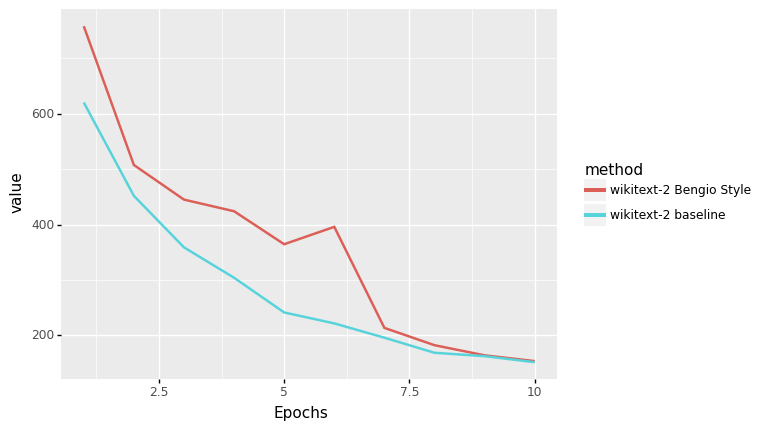
\includegraphics[height=10cm]{Thesis/images/wikitext-2BS.png}
\caption{Validation perplexity of baselines and replacement methods trained on wikitext-2 measured every epoch.}
\label{fig:cs-perp-2}
\end{figure}
\begin{figure}[h]
\centering
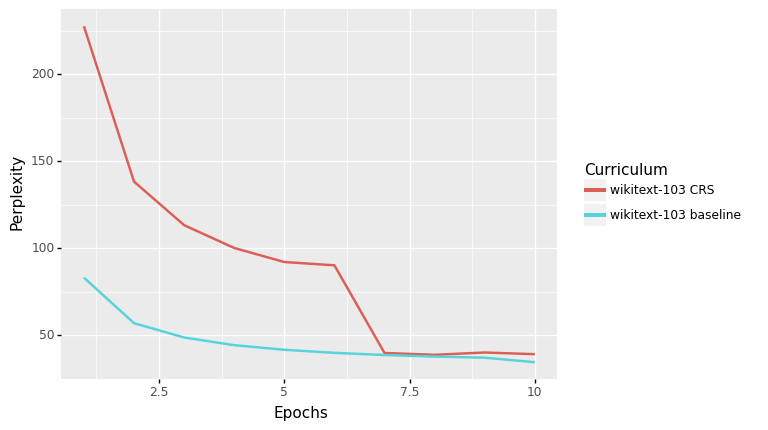
\includegraphics[height=10cm]{Thesis/images/wikitext-103BS.png}
\caption{Validation perplexity of baselines and replacement methods trained on wikitext-103 measured every epoch.}
\label{fig:cs-perp-103}
\end{figure}
\begin{table}[]
\resizebox{\textwidth}{!}{%
\begin{tabular}{|l|l|l|l|l|l|l|l|l|l|l|l|}
\hline
Method & \textbf{Overall Score} & Cola & SST & MRPC & STS-B & QQP & MNLI & QNLI & RTE & WNLI & DX \\ \hline
Baseline wiki103 & \textbf{0.671} & \textbf{0.281} & \textbf{0.862} & 0.866/0.801 & 0.765/0.773 & 0.716/0.763 & 0.644 & \textbf{0.761} & \textbf{0.610} & 0.535 & 0.139 \\\hline
CRS wiki103 & 0.657 & 0.254 & 0.852 & \textbf{0.875}/\textbf{0.816} & \textbf{0.794}/\textbf{0.793} & \textbf{0.738}/\textbf{0.785} & 0.662 & 0.719 & 0.588 & 0.437 & \textbf{0.162} \\\hline
Baseline wiki2 & 0.607 & 0.06 & 0.742 & 0.854/0.789 & 0.683/0.684 & 0.697/0.745 & 0.566 & 0.726 & 0.581 & \textbf{0.563} & 0.119 \\\hline
CRS wiki2 & 0.59 & 0 & 0.7 & 0.846/0.775 & 0.661/0.663 & 0.701/0.753 & 0.585 & 0.717 & 0.542 & \textbf{0.563} & 0.13 \\\hline
Baseline BWC & 0.595 & 0 & 0.852 & 0.823/0.711 & 0.547 & 0.733/0.765 & \textbf{0.671} & 0.719 & 0.48 & \textbf{0.563} & 0.155 \\ \hline
\end{tabular}%
}
\caption{GLUE results for competence replacement methods and baselines trained on wikitext-2.}
\label{table:glue-corpus}
\end{table}
The effect of the curricula looking at GLUE can be found in Table \ref{table:glue-corpus}. First, we find that the pubic ELMo implementation performs worse on the GLUE dataset than all of our implementations. It is unclear why this is, and we will not focus on this further. Next, we see that when the training corpus is small, the BS implementation outperforms the baseline method by a sizable margin. As the corpus size grows, the baseline performance passes all other methods. There is high variability in individual task scores such that STS-B and the Diagnostic tests are much better with the BS system, while COLA, WNLI, and RTE are much better in the baseline method. One possible cause of this is BS models learn better representations for binary classifications but not better representations for multi-label classification. If we exclude WNLI, the BS methods outperform the baseline methods by a wide margin. We can also observe various tasks that the small corpus models cannot learn as both wiki2 models achieve 0 on COLA. We believe this may result from the model learning a flipped representation early on and not being able to recover from it. There does not seem to be a clear association in curriculum methods performing worse or better based on the task training data size. On some tasks with small training corpus like RTE the non curriculum methods perform better while in others like STS-B the top model is a CRS method.
\section{Competence-Based Curricula}
\subsection{Wikitext-2}
Looking at performance on the small corpus in Figure 4.3 and Figure 4.4 we see that all the curricula methods start to overfit on the training corpus after about 16 of the 24 epochs (which equates to when the curriculum training is finished). The full data underpinning the figures mentioned above can be found in the Appendix. Despite seeing over-fitting, we see that POS and DEP generally learn some of the lowest perplexity on the validation set. Looking at the difference between sentence-level and line-level training, we see a closer grouping in model performance distribution between sentence vs. line, which we attribute to a common sentence-level structure independent to corpus separation. Finally, we see that the best performance is achieved by the non-curricula baseline (initial competence set to 1) with a perplexity of 770, followed by Random with a perplexity of 2105. Despite the success of these curriculums, all are orders of magnitude above the baseline score of 151. We believe this is caused by the change in dataset distribution caused by our curriculum learning implementation. Even our baseline curricula which has access to the full training corpus does not achieve a high perplexity as the distribution it sees in training differs from the true distribution. \\
As we move our focus to GLUE results as shown in Table \ref{tab:wiki2-glue}, we see a very different picture as the curriculum methods generally outperform the baselines by a wide margin. We see that models do not seem to learn any representation that can be used by WNLI, as those results are all virtually identical. Surprisingly it does not seem that a more optimal method for splitting the corpus is apparent as sentence-based training achieves a similar result in line-based training. We believe this means we cannot make a strong generalization that can be made about the effects of what method is used for training. The final point to observe is that nearly every curricula method outperforms the baseline implementation. Perhaps most surprising, random curricula performing second best when measure by overall glue score despite their being no motivation to the structure the model sees. \\
Overall, when training on wiki2, we find that competency-based curricula methods provide somewhat of a mixed message. While performance on the validation portion is much worse, GLUE performance is much better. Since we believe what is most important in a model is how well the language representations can transfer to downstream tasks, we argue that with small training datasets CBC outperform traditional training regimes.
\begin{figure}[H]
\centering
\label{fig:wk2lp}
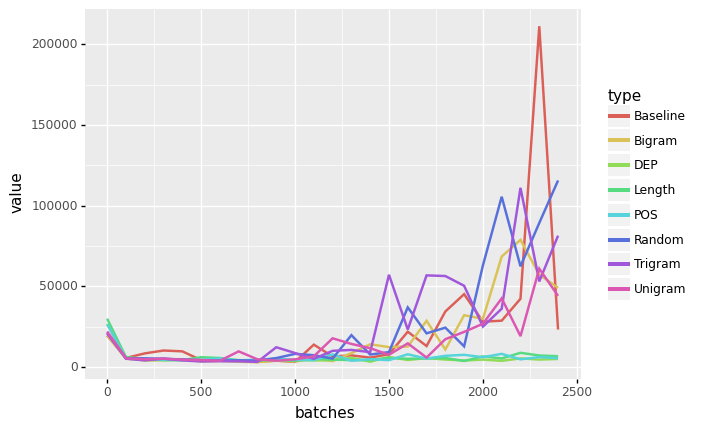
\includegraphics[ height=10cm]{Thesis/images/wikitext-2line.png}
\caption{Validation perplexity of each curriculum trained on line based wikitext-2 measured every 100 batches.}
\end{figure}
\begin{figure}[H]
\centering
\label{fig:wk2spy}
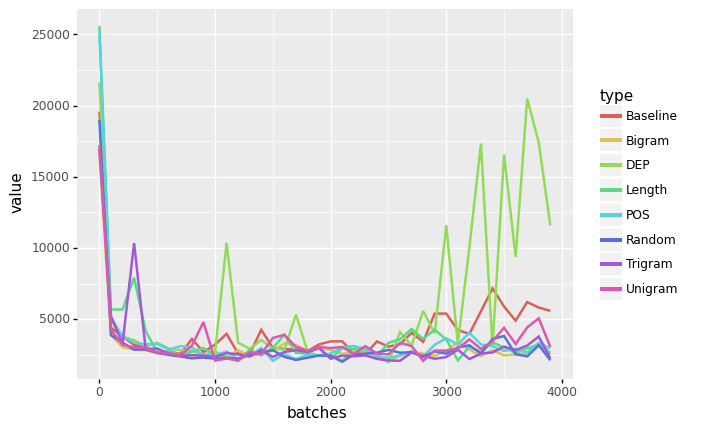
\includegraphics[ height=10cm]{Thesis/images/wikitext-2sentence.png}
\caption{Validation perplexity of each curriculum trained on sentence based wikitext-2 measured every 100 batches.}
\end{figure}
\begin{table}[h]
\resizebox{\textwidth}{!}{%
\begin{tabular}{|l|l|l|l|l|l|l|l|l|l|l|l|}
\hline
Method & Overall & Cola & SST & MRPC & STS-B & QQP & MNLI & QNLI & RTE & WNLI & DX \\\hline
bigram-s & \textbf{0.645} & \textbf{0.188} & 0.790 & 0.844/0.775 & \textbf{0.732/0.733} & 0.742/0.788 & 0.617 & 0.766 & 0.570 & \textbf{0.563} & 0.131 \\ \hline
random-s & 0.644 & 0.210 & 0.780 & 0.847/0.779 & 0.715/0.712 & \textbf{0.744}/0.791 & \textbf{0.616} & 0.760 & 0.570 & \textbf{0.563} & 0.143 \\ \hline
unigram-s & 0.640 & 0.209 & 0.755 & 0.861/\textbf{0.799} & 0.731/0.731 & 0.733/0.778 & 0.613 & 0.757 & 0.545 & \textbf{0.563} & 0.135 \\ \hline
pos-s & 0.637 & 0.207 & 0.765 & 0.849/0.777 & 0.714/0.714 & 0.727/0.781 & 0.606 & 0.745 & 0.567 & \textbf{0.563} & 0.134 \\ \hline
dep-s & 0.636 & 0.175 & \textbf{0.792} & \textbf{0.863}/0.797 & 0.721/0.720 & 0.727/0.786 & 0.613 & 0.749 & 0.567 & \textbf{0.521} & 0.137 \\\hline
dep-l & 0.632 & 0.190 & 0.727 & 0.85/0.782 & 0.708/0.704 & 0.735/0.782 & 0.598 & \textbf{0.748} & 0.581 & \textbf{0.563} & 0.118 \\\hline
unigram-l & 0.628 & 0.175 & 0.768 & 0.856/0.782 & 0.675/0.674 & 0.738/0.792 & 0.598 & 0.746 & 0.560 & \textbf{0.549} & 0.132 \\ \hline
trigram-l & 0.627 & 0.152 & 0.761 & 0.838/0.762 & 0.695/0.691 & 0.730/0.782 & 0.616 & 0.764 & 0.542 & \textbf{0.563} & 0.144 \\\hline
trigram-s & 0.626 & 0.172 & 0.788 & 0.833/0.779 & 0.730/0.731 & \textbf{0.744/0.796} & 0.620 & 0.761 & 0.552 & 0.437 & \textbf{0.137} \\\hline
length-l & 0.625 & 0.185 & 0.748 & 0.844/0.770 & 0.658/0.654 & 0.725/0.783 & 0.601 & 0.748 & 0.567 & \textbf{0.563} & 0.128 \\ \hline
no curricula-s & 0.621 & 0.148 & 0.747 & 0.836/0.770 & 0.706/0.705 & 0.734/0.780 & 0.612 & 0.719 & 0.538 & \textbf{0.563} & 0.121 \\\hline
bigram-l & 0.616 & 0.175 & 0.768 & 0.856/0.782 & 0.675/0.674 & 0.738/0.792 & 0.598 & 0.746 & 0.560 & \textbf{0.437} & 0.132 \\\hline
random-l & 0.614 & 0.000 & 0.763 & 0.847/0.775 & 0.699/0.699 & 0.721/0.784 & 0.611 & 0.749 & 0.578 & \textbf{0.563} & 0.143 \\\hline
CRS & 0.607 & 0.060 & 0.742 & 0.854/0.789 & 0.683/0.684 & 0.697/0.745 & 0.566 & 0.726 & 0.581 & \textbf{0.563} & 0.119 \\\hline
pos-l & 0.607 & 0.000 & 0.737 & 0.842/0.770 & 0.663/0.660 & 0.712/0.771 & 0.610 & 0.750 & 0.592 & \textbf{0.563} & 0.155 \\\hline
no curricula-s & 0.591 & 0.069 & 0.768 & 0.847/0.765 & 0.728/0.731 & 0.722/0.758 & 0.500 & 0.718 & 0.538 & 0.451 & 0.107 \\\hline
base & 0.590 & 0.000 & 0.700 & 0.846/0.775 & 0.661/0.663 & 0.701/0.753 & 0.585 & 0.717 & 0.542 & \textbf{0.563} & 0.130 \\\hline
length-s & 0.528 & -0.006 & 0.750 & 0.805/0.674 & 0.708/0.710 & 0.537/0.682 & 0.326 & 0.510 & \textbf{0.592} & 0.521 & 0.008 \\ \hline
\end{tabular}%
}
\caption{GLUE results for competence based curricula methods on trained on wikitext-2.}
\label{tab:wiki2-glue}
\end{table}

\subsection{wikitext-103}
As we scale to the larger corpus, we find that not all the trends seen on the small data hold. Looking at the results in Figure 4.5, Figure 4.6 and Figure 4.7, we can see that similar to the smaller corpus, none of the curriculum learned models can learn a representation that transfers from their perturbed training to the validation set. Unlike the non-curriculum techniques, which achieve a perplexity of 36, none of the curricula methods ever learn a model with a perplexity under one thousand. We note that similar to what was seen on the wiki2 is on wiki103. N-gram methods have a similar distribution in performance. Also, holding over from wiki2, DEP, LEN, and POS demonstrates a slow and steady improvement in perplexity as their training continues. As the dataset has grown larger, we see increased volatility in perplexity changes across all training methods.\\
Looking at the result of the transfer tasks in Table \ref{tab:glue-wiki-103}, we find that the trends we see in the smaller corpus no longer hold. The best model in terms of transfer learning is the non-curriculum baseline implementation from the original ELMo implementation. This baseline method outperforms on the overall score and outperforms every other model on tasks like CoLA, where the score is nearly 20\% better. Surprisingly, after the baseline method, the trigram curricula appear to generate the best transfer task as both sentence and line-based methods as they are ranked second and third when measured on the average across tasks. We also note that some of the best performing curricula are also those models that had some of the highest perplexities on the training task. \\
\begin{figure}[H]
\centering
\label{fig:wikitext103-line}
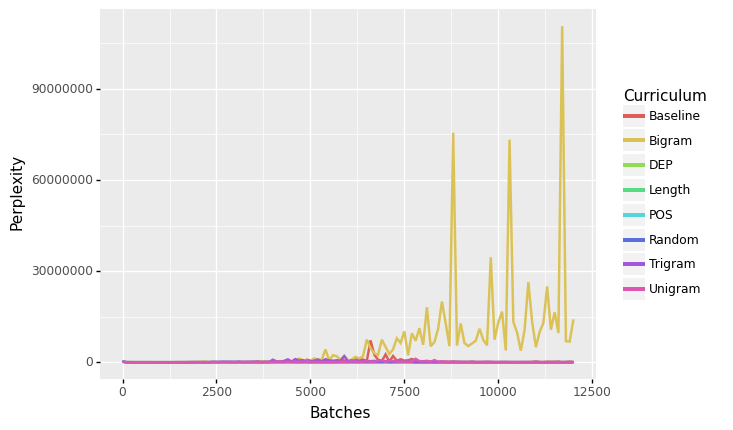
\includegraphics[height=10cm]{Thesis/images/wikitext-103lineall.png}
\caption{Validation perplexity of each curriculum trained on line based wikitext-103 measured every 100 batches.}
\end{figure}
\begin{figure}[H]
\centering
\label{fig:wikitext103-line-clean}
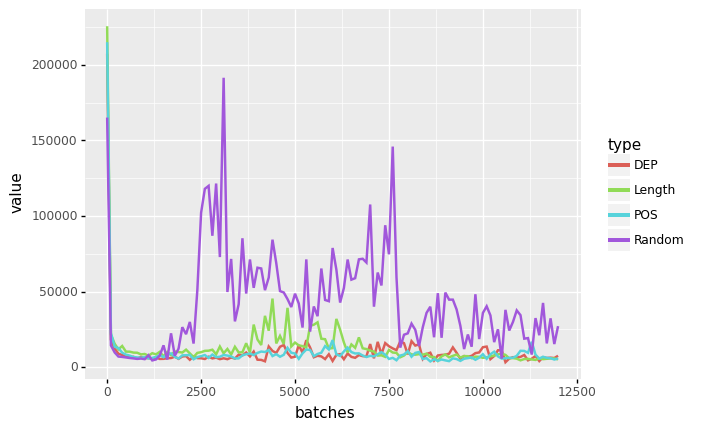
\includegraphics[height=10cm]{Thesis/images/wikitext-103lineminusbigrambaselinetrigramunigram.png}
\caption{Validation perplexity of each curriculum trained on line based wikitext-103 measured every 100 batches. Unigram, bigram, and baseline model performance removed improved interpretation}
\end{figure}
\begin{figure}[H]
\centering
\label{fig:wikitext103-sentence}
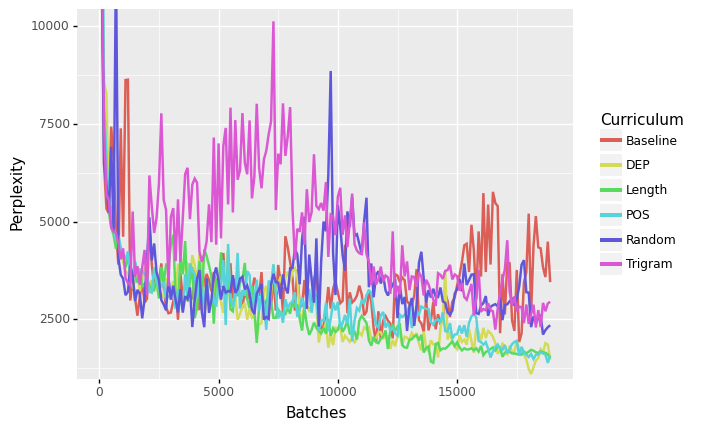
\includegraphics[ height=10cm]{Thesis/images/wikitext-103sentenceminusbigramunigram.png}
\caption{Validation perplexity of each curriculum trained on sentence based wikitext-103 measured every 100 batches.}
\end{figure}
\begin{table}[]
\centering
\resizebox{\textwidth}{!}{%
\begin{tabular}{|l|l|l|l|l|l|l|l|l|l|l|l|}
\hline
Method & Overall & Cola & SST & MRPC & STS-B & QQP & MNLI & QNLI & RTE & WNLI & DX \\\hline
baseline & \textbf{0.671} & \textbf{0.281} & \textbf{0.862} & 0.866/0.801 & 0.765/0.773 & 0.716/0.763 & 0.644 & 0.761 & 0.610 & 0.535 & 0.139 \\\hline
trigram-s & 0.666 & 0.208 & 0.857 & 0.865/0.806 & 0.790/0.790 & 0.733/0.779 & \textbf{0.658} & 0.757 & 0.567 & \textbf{0.563} & 0.136 \\\hline
trigram-l & 0.665 & 0.207 & 0.854 & 0.871/0.804 & 0.781/0.782 & 0.752/\textbf{0.799} & 0.655 & 0.767 & 0.556 & 0.549 & 0.144 \\\hline
unigram-s & 0.664 & 0.190 & 0.856 & 0.861/0.797 & 0.784/0.784 & 0.747/0.791 & 0.654 & 0.773 & 0.556 & \textbf{0.563} & 0.140 \\\hline
no curriculum-s & 0.663 & 0.190 & 0.845 & \textbf{0.878/0.824} & 0.767/0.768 & 0.748/0.788 & 0.651 & 0.746 & 0.588 & \textbf{0.563} & 0.140 \\\hline
no curriculum-l & 0.663 & 0.214 & 0.826 & 0.865/0.804 & 0.766/0.766 & 0.747/0.789 & 0.643 & \textbf{0.772} & 0.581 & \textbf{0.563} & 0.145 \\\hline
random-s & 0.661 & 0.203 & 0.843 & 0.870/0.806 & 0.778/0.779 & 0.740/0.789 & 0.644 & 0.745 & 0.574 & \textbf{0.563} & 0.151 \\ \hline
length-s & 0.659 & 0.229 & 0.827 & 0.867/0.804 & 0.765/0.766 & 0.747/0.783 & 0.642 & 0.762 & 0.538 & \textbf{0.563} & 0.135 \\\hline
CRS & 0.657 & 0.254 & 0.852 & 0.875/0.816 & \textbf{0.794/0.793} & 0.738/0.785 & 0.662 & 0.719 & 0.588 & 0.437 & \textbf{0.162} \\\hline
bigram-l & 0.656 & 0.180 & 0.826 & 0.854/0.792 & 0.770/0.770 & 0.753/0.794 & 0.645 & 0.766 & 0.560 & \textbf{0.563} & 0.137 \\\hline
length-l & 0.656 & 0.212 & 0.820 & 0.851/0.782 & 0.768/0.767 & 0.734/0.788 & 0.634 & 0.752 & 0.578 & \textbf{0.563} & 0.135 \\\hline
unigram-l & 0.654 & 0.194 & 0.823 & 0.857/0.789 & 0.755/0.754 & 0.752/0.794 & 0.625 & 0.753 & 0.574 & \textbf{0.563} & 0.125 \\ \hline
random-l & 0.652 & 0.179 & 0.836 & 0.861/0.789 & 0.772/0.774 & 0.753/0.797 & 0.640 & 0.772 & 0.578 & 0.493 & 0.139 \\\hline
pos-l & 0.649 & 0.163 & 0.827 & 0.861/0.794 & 0.756/0.757 & \textbf{0.754}/0.791 & 0.630 & 0.732 & 0.570 & \textbf{0.563} & 0.138 \\ \hline
bigram-s & 0.649 & 0.195 & 0.859 & 0.867/0.799 & 0.784/0.785 & 0.736/0.772 & 0.651 & 0.754 & 0.599 & 0.408 & 0.132 \\\hline
dep-l & 0.644 & 0.231 & 0.846 & 0.856/0.779 & 0.776/0.776 & 0.746/0.786 & 0.637 & 0.761 & 0.542 & 0.423 & 0.137 \\ \hline
pos-s & 0.640 & 0.114 & 0.794 & 0.853/0.772 & 0.775/0.774 & 0.740/0.782 & 0.624 & 0.738 & 0.578 & \textbf{0.563} & 0.108 \\ \hline
dep-l & 0.587 & -0.040 & 0.842 & 0.805/0.679 & 0.786/0.789 & 0.682/0.730 & 0.321 & 0.757 & \textbf{0.614} & 0.549 & 0.038 \\ \hline
\end{tabular}%
}
\caption{GLUE results for Competence based curricula methods on trained on wikitext-103.}
\label{tab:glue-wiki-103}
\end{table}
\section{Discussion}
Reflecting on our experiments and questions posed earlier in the dissertation in Section \ref{chap:method} we believe our results support the following findings:
\begin{enumerate}
\item CL can help converge to a more optimal global minima when the training corpus is small. As corpus size scales, the positive impact of CL disappears.
\item The downstream representation learned via CL outperforms non-curricula methods when the corpus size is small, but as the corpus size grows, CL methods no longer generate the best representation.
\item CL methods do not help the model convergence speed in any noticeable way and in our use of padding tokens CL methods actually make training fare less efficient than non CL methods.
\end{enumerate}
These finding, matched with no generalized superior curricula performance and the increased cost in running curriculum methods lead us to believe that language models learn more from the stochastic sampling of a corpus than any structure experimenters try to introduce. 
\subsection{Failure of Competence Based Curriculum}
What surprised us most in our results was the failure in learning the training data we see in our CBC method. Based on the changes in validation perplexity we believe the model is over-fitting on the altered training data. We believe the cause of this is our hyperparameter selection for $\lambda_0$ and $\lambda_{increment}$. We realize that since each method is effusively sampling from a different training distribution comparison of training perplexities are not comparable. Additionally, if we look at the difference in validation perplexity curves of various methods it is apparent that they are not learning at the same rate. Some methods like DEP, and POS do not see major fluctuations indicating the chosen curriculum parameters work well while many of the $n$-gram methods consistently fluctuate in a similar fashion indicating the chosen hyperparameters are sub optimal for them. Given the non trivial computational cost to explore $\lambda_0$ and $\lambda_{increment}$ for each method and the disconnect seen between pre-training perplexity and performance on GLUE we have decided to to pursue further optimization in this dissertation.
\subsection{Curriculum Learning Alters the Data Distribution}
We find it useful to formulate CL as moving from sampling without replacement to sampling with replacement with an ever-growing population. As a result, our implementations of CBC do not guarantee that the model will see the entire dataset ten times, and as a result, the distribution of the data seen in training is likely different from the distribution of the validation dataset. We believe this is why the CL implementations can never generalize their performance in the train portion of the corpus to the validation portion. To avoid this one such approach would be to over sample easy portions of the training data in early training and extend the length of this epoch. This way the model could build of easy example but still see every part of the training corpus at least ten times. \\
Despite this inability to learn the training distribution, CBC methods are still able to transfer well to understanding tasks, which makes us think that what is important in pre-training is not the actual task but what the model can learn from the task. This finding is interesting because it challenges the notion that a model must fit the target dataset well to learn a representation that transfers well to downstream tasks. We find that even the models with high validation perplexities can still learn good representations for our transfer task. \\
Another observation our data leads us to is tweaking the training distribution's can allow the models to do better in transfer tasks because it is unable to overfit to the small pre-training corpus. Since our implementation generates some form of continually changing data distribution from where random batches are sampled, the train distribution is continually changing. Since the training regime is constantly changing, we hypothesis CBC is effectively simulating a larger, more complex dataset. On one hand, this larger artificial training set causes the model never learns a good representation of the original training corpus which we see in model perplexity. On the other hand, since the model never learns a good representation of the training corpus it can effectively simulate a much larger training corpus which produces a LR which when measured in terms of transfer performance is much better. This is especially apparent in the effectiveness of random curricula, where the random training structure still leads to improved transfer performance. Instead of having one consistent dataset of size $N$ we have a dataset of $size = \sum_{t=0} N * \lambda_t$ datasets.  \\
Independently of what heuristic is used in early training, some portion (usually the easy portion) is over-sampled while in other portions (usually hard portion), examples are under-sampled. Recently, work in understanding how NN work has lead to the discovery there are sub-networks within the larger NN, which are more optimal for the task \cite{Frankle2019TheLT}. The process of training a DNN can be thought of as an architecture search within the larger randomly initiated network by decreasing the weights of sub-optimal sub-networks and increasing the weights of optimal sub-networks. Since the CL method is oversampling some portion of the dataset during early training, CL methods will favor sub-networks that are likely not optimal for the full data distribution. We believe this may be the cause of why CL methods under-perform non-CL methods on the training task. One way to address this shortcoming would be to modify curricula methods to create ever-changing distributions that are close to the original distribution. In other words, in early training, instead of oversampling from the lower strata of the CDF CL methods could sample from slightly distorted distributions of the same CDF. One such implementation may divide the data into deciles and sample from each decile for each epoch. In other words instead of sampling from the whole distribution the first training epoch would sample from the lowest 10\% of the CDF while the last training epoch would sample from the highest 10\%. 
\subsection{Training Efficiency}
With regard to improving the efficiency of LM training, our implementations had the opposite effect. Our implementation of CBC introduces an overhead which makes training over 40\% less efficient. In seeing the effective impact of successful training datasets like the Toronto Book corpus we believe that successful CL methods need to focus on rebalancing training distribution in a model independent method. By rebalancing data distributions CL methods can ensure that the cost of compute only happens once instead of the $n$ times the data is resampled in model training and the $m$  potential models that use this data. Moreover, by moving curriculum generation outside of model training CL methods can have a larger impact because researchers only need to train on a new dataset instead of changing their model code. \\
\subsection{Sentence vs Line Training}
We find No marked difference in the effects of training with sentence-based vs line based corpora when evaluated on GLUE. We do find a large difference in perplexity on the pre-training task but we believe this is caused by the inefficiency introduced by our padding token. Since sentence based sampling has ~30\% more padding tokens the model is able to learn substantially less from every sample when compared to the line corpus. Surprisingly this decreased ability to learn the training data seems to have no impact on transfer performance. This is in line with the purpose of pretraining as the goal is not actually to learn the training data but use it to form a generalized representation. 
\chapter{Conclusion}
Throughout this thesis we have explored how some approaches in curriculum learning apply to language modeling. In our research we explored 2 types of curricula and applied them to the pretraining of ELMO, a language model. Our first curricula(previously referred to as Bengio Style) makes the training corpus more difficult by limiting the training vocabulary in regularly spaced increments. This curricula is not able to improve model perplexity on the training corpus but when the corpus is small outperforms the non curricula methods on transfer tasks and as the corpus scales improves the performance on a subset of NLP applications. Our second curricula method(previously referred to as competence curricula) explores the effect of various curricula when applied to the same language model pretraining. In these experiments we find that while the model cannot learn a good representation of the training corpus the representations they transfer downstream NLP tasks prove to be resilient. We find that on small corpuses competence curricula show improvement versus non curricula method across the board. As we scale the corpus size we find that non curricula methods out perform all curricula. We do not find any superiority in the curricula we explore nor do we find a compelling difference in the effects of training with sentences over lines. While our implementations were not able to produce improvements we believe the results set the stage for further research and poses some broader questions for learning methods for NN in general. 
\chapter{Future Work}
\label{chap:future}
We seek to continue our exploration of CL methods and methods to make training and using models more efficient in the future. Since we began our work there has been much exciting work on finding sub-networks in NN that preserve the accuracy of the original model \cite{Frankle2019TheLT}. Other methods have explored the pruning of large models for smaller equally accurate models \cite{Han2016DeepCC} \cite{Yu2017ScalpelCD} \cite{Wynter2020OptimalSE} which we would like to expand on, focusing on how these pruning methods perform with transfer learning. Additionally, inspired by the layered nature of Transformer-based models, we would explore jointly how progressive methods may look like for LMs. One such approach would be to increase the number of transformer encoders while increasing data difficulty, similar to what has been done with GANs \cite{Karras2017ProgressiveGO}. Another method may model longer context windows progressively starting in short sentences and reaching entire documents. Finally, in the future, we seek to make a benchmarking system that can allow authors to explore the effect of various curricula on many downstream tasks. If the broader community had an easy to use a benchmark, they could focus on studying the overall impact of curricula.  The goal would be to provide a framework similar to GLUE and JIANT, which provide a set of architectures and tasks which would allow researchers to focus only on sampling methods.
\printendnotes
\nocite{*}
\bibliographystyle{plain}
\bibliography{uwthesis}
\appendix
\raggedbottom\sloppy
\vita{Daniel Campos is a PhD student at the University of Illinois Urbana-Champaign where he is working on next generation NLP systems focused on chemistry and agriculture. {\tt spacemanidol@gmail.com}.}
\end{document}
